190. \begin{figure}[ht!]
\center{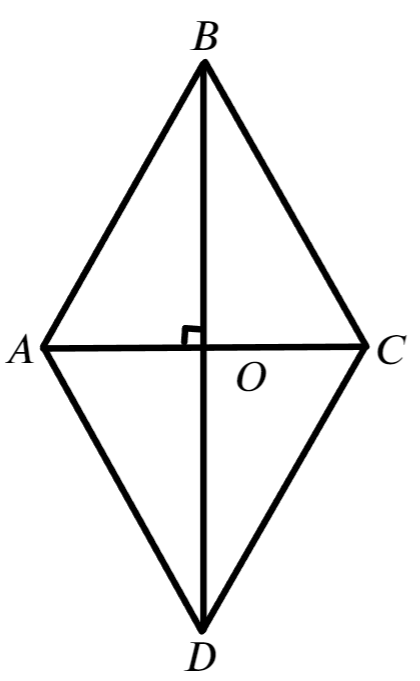
\includegraphics[scale=0.35]{g9-190.png}}
\end{figure}\\
В ромбе диагонали перпендикулярны и делятся точкой пересечения пополам, поэтому\\ $BO=\sqrt{17^2-8^2}=15,\ BD=30.$ Тогда $S=\cfrac{1}{2}\cdot16\cdot30=r\cdot\cfrac{4\cdot17}{2},$ откуда $r=\cfrac{120}{17}.$\\
